\documentclass[./project-report/src/latex/project-report.tex]{subfiles}

\begin{document}

\maketitle

\clearpage

\section{Investigation}

This section outlines the code utilised to test the performance of a trained network. It then utilises this functionality to explore the effects of Hyper-Parameters on the 
Artificial Neural Network performance.

\subsection{test\_model module}
\label{sec:test_model-module}

The test\_model module is contained within the frames package, and contains tkinter frames for testing the trained Artificial Neural Network models for each dataset. 
For each training dataset that an Artificial Neural Network is trained on, there is a corresponding test dataset with completely new images to be tested on to judge 
the performance of the trained model. As fewer images are needed for testing than for training, the Cat dataset only has 50 test images (compared to the 209 images 
for training) and the MNIST dataset only has 10,000 test images (compared to the 60,000 images for training).
Each frame displays the results of the testing along with a random selection of incorrect and correct predictions.

\inputminted{python}{./school_project/frames/test_model.py}

Which outputs the following results depending on the dataset used:

\pagebreak

\begin{figure}[h!]
\centering
\frame{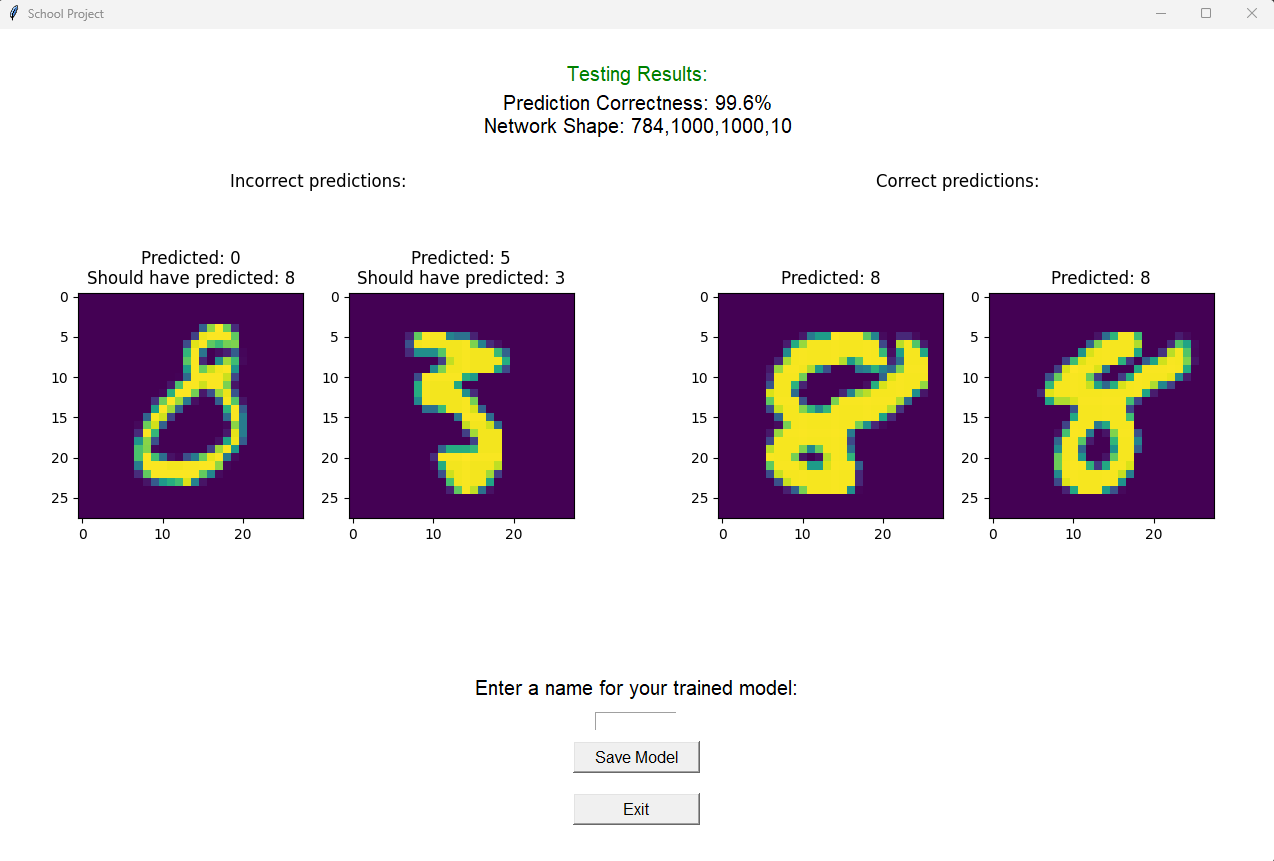
\includegraphics[width=1\textwidth]{./project-report/src/images/test-mnist-frame.png}}
\caption{Model test results for MNIST database}
\label{fig:test-frame-impl}
\end{figure}

\pagebreak

\begin{figure}[h!]
\centering
\frame{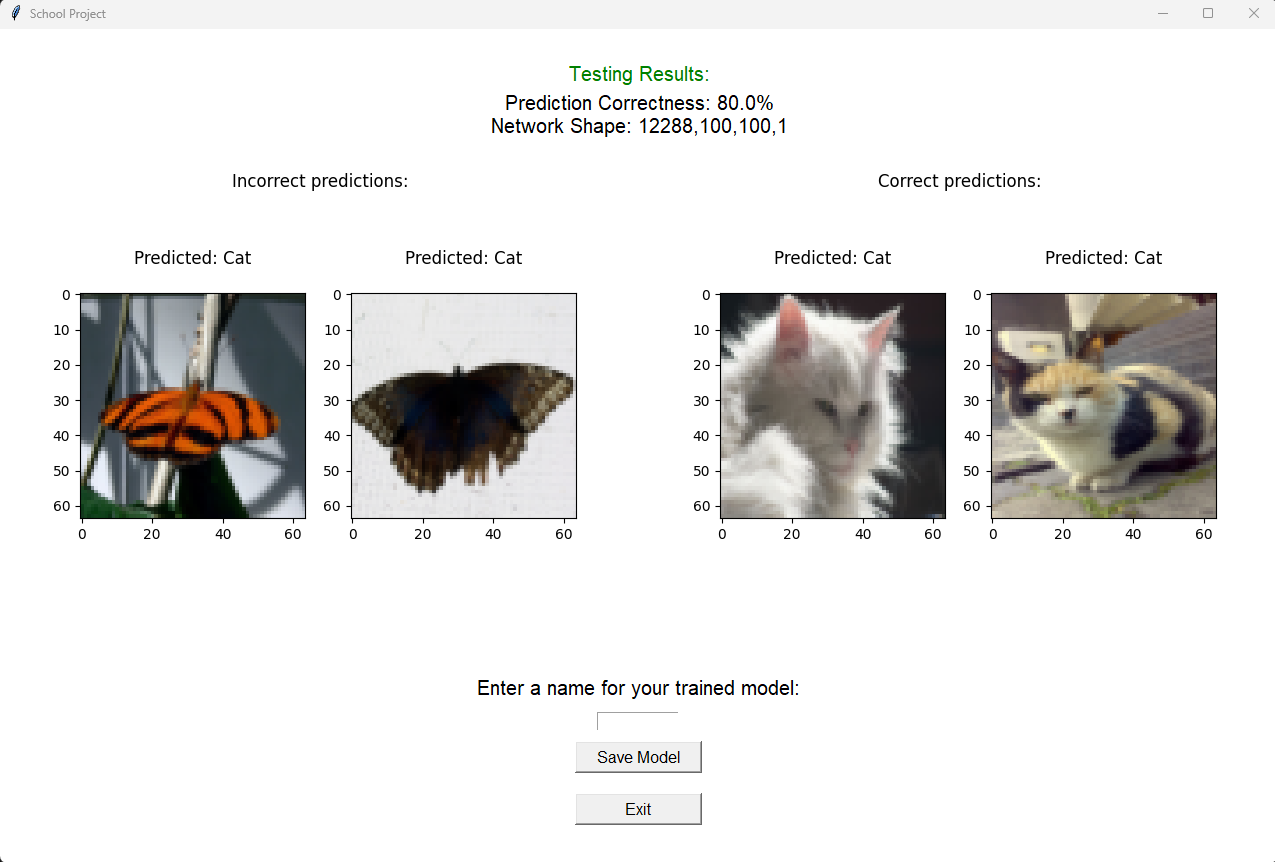
\includegraphics[width=1\textwidth]{./project-report/src/images/test-cat-recognition-frame.png}}
\caption{Model test results for Cat recognition database}
\end{figure}

\pagebreak

\begin{figure}[h!]
\centering
\frame{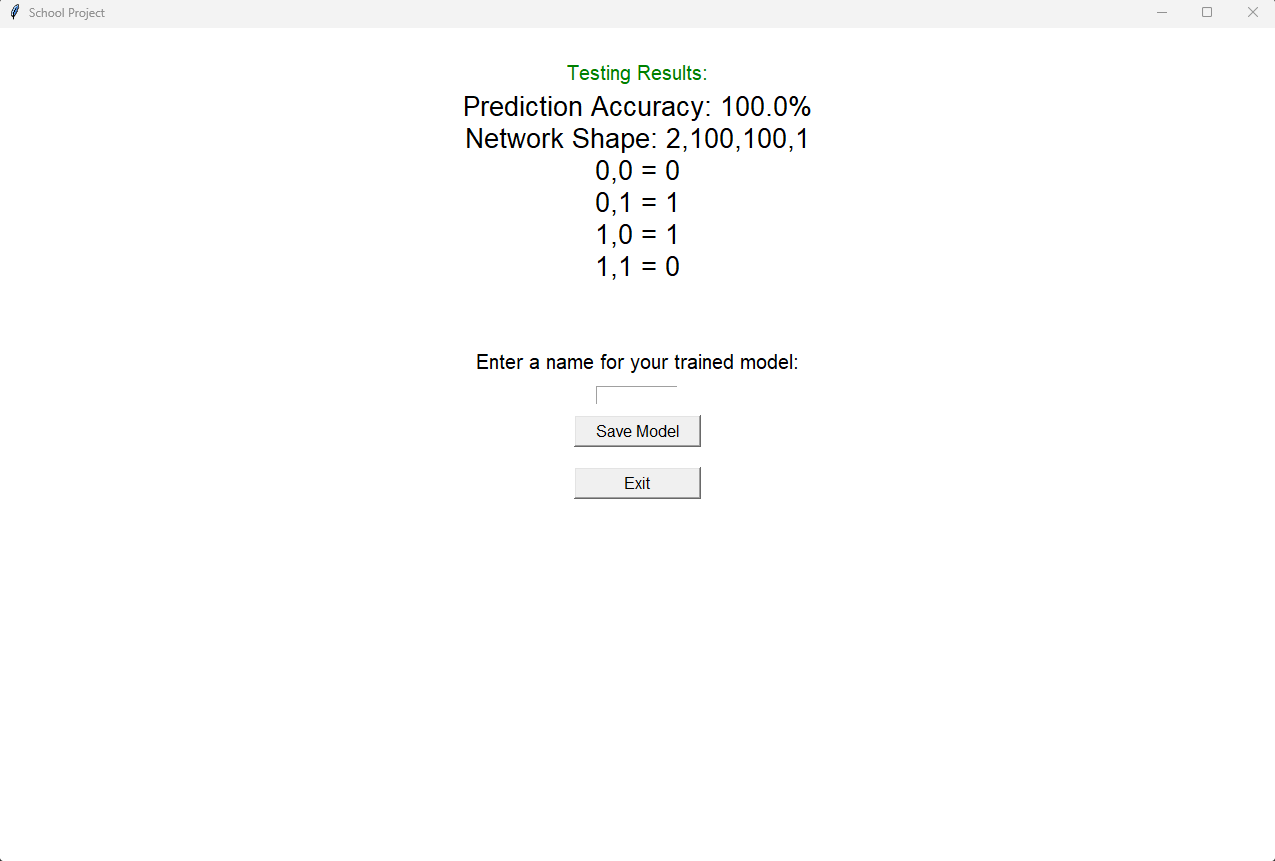
\includegraphics[width=1\textwidth]{./project-report/src/images/test-xor-frame.png}}
\caption{Model test results for XOR dataset}
\end{figure}

\subsection{Effects of Hyper-Parameters}
\label{sec:effects-of-hyper-parameters}

As discussed in section \ref{sec:ann-theory} Artificial Neural Networks have a number of critical hyper-parameters which describe the shape of the network and the nature in 
which it learns. To explore this, I have conducted a series of experiments utilising the program to explore the fundamental impact of these hyper-parameters. In particular I 
explored the impact of the:

\begin{itemize}
    \item Learning rate
    \item Number of Epochs undertaken during training
    \item Training dataset size
    \item Number of hidden layers
    \item Number of neurons in each layer
    \item Use of the ReLu vs Sigmoid transfer function
    \item Use of GPU vs CPU 
\end{itemize}

For these investigations, I utilised Jupyter Notebook to run blocks of code and display the results. The output of each Jupyter Notebook is shown in the 
analysis below.

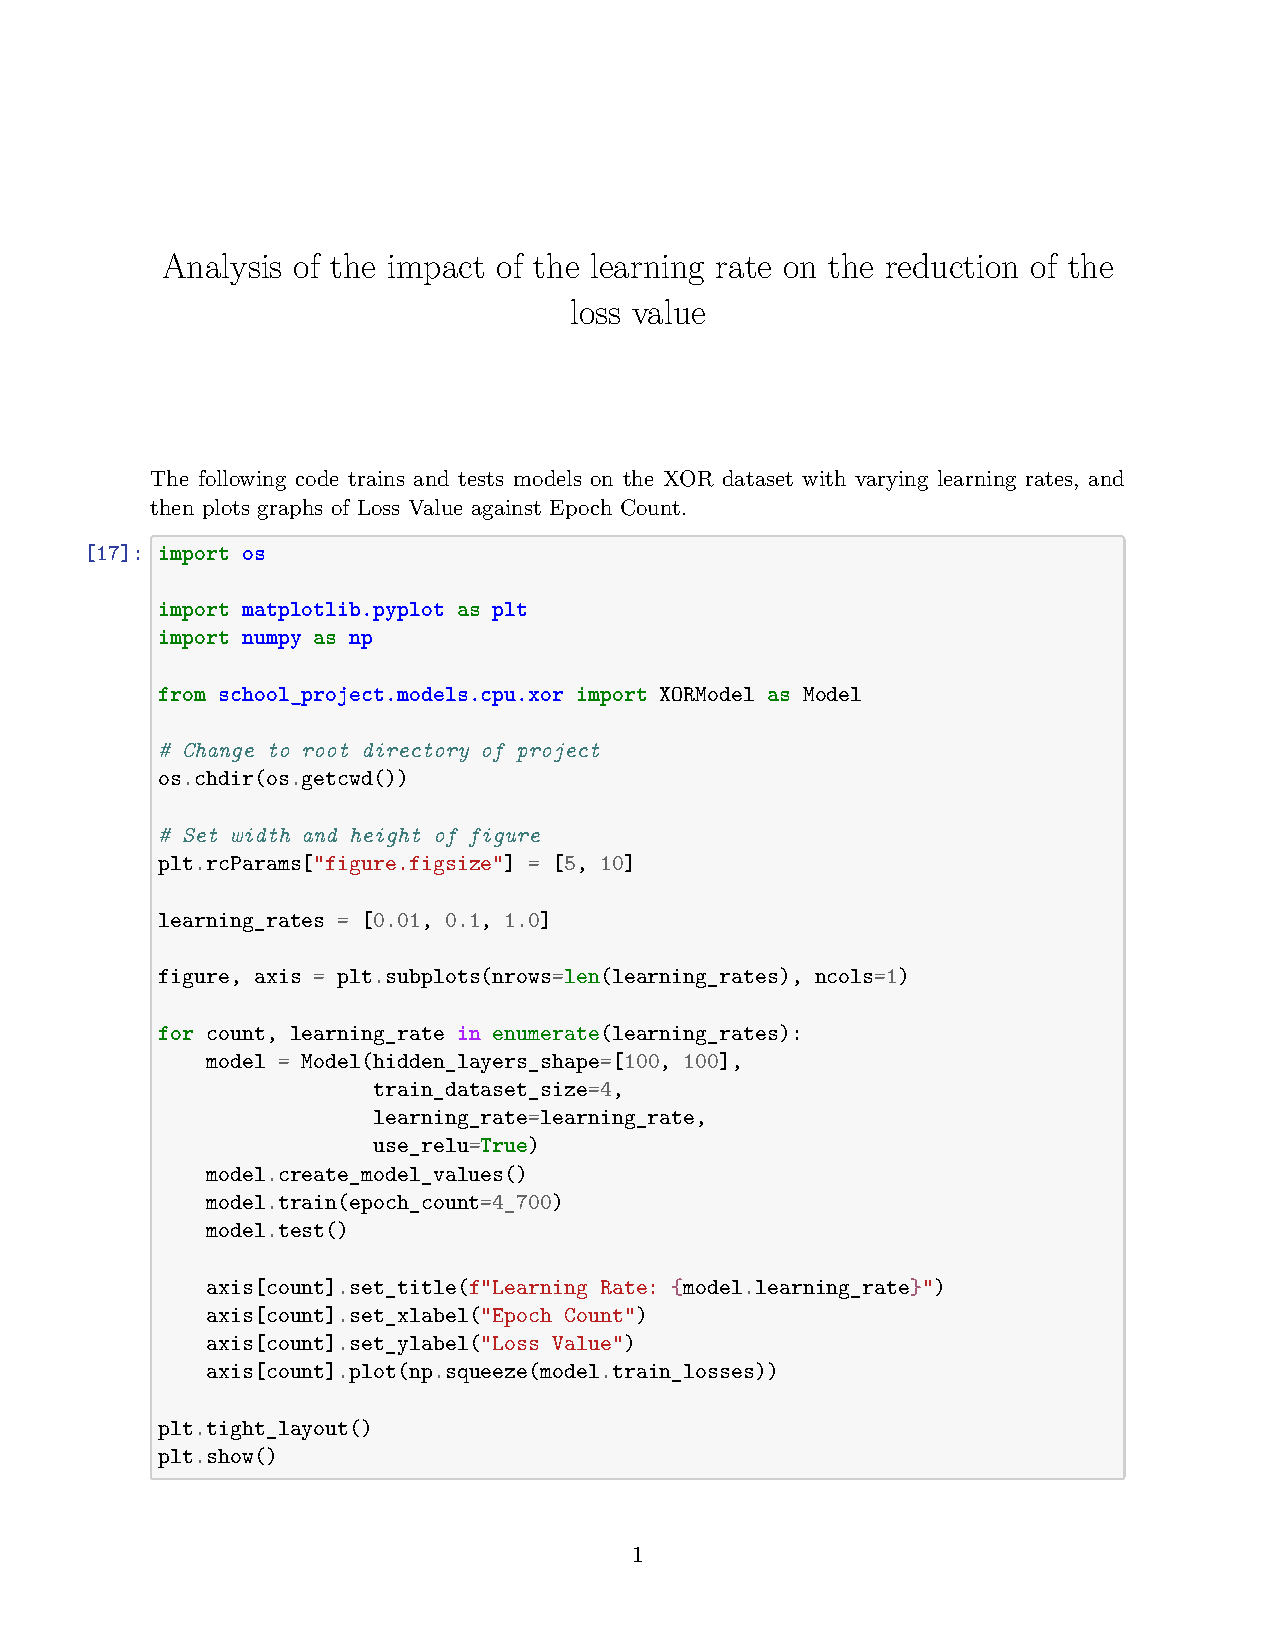
\includepdf[pages=-, pagecommand={\thispagestyle{plain}}, scale=0.9]{./project-report/src/pdfs/learning-rate-analysis.pdf}

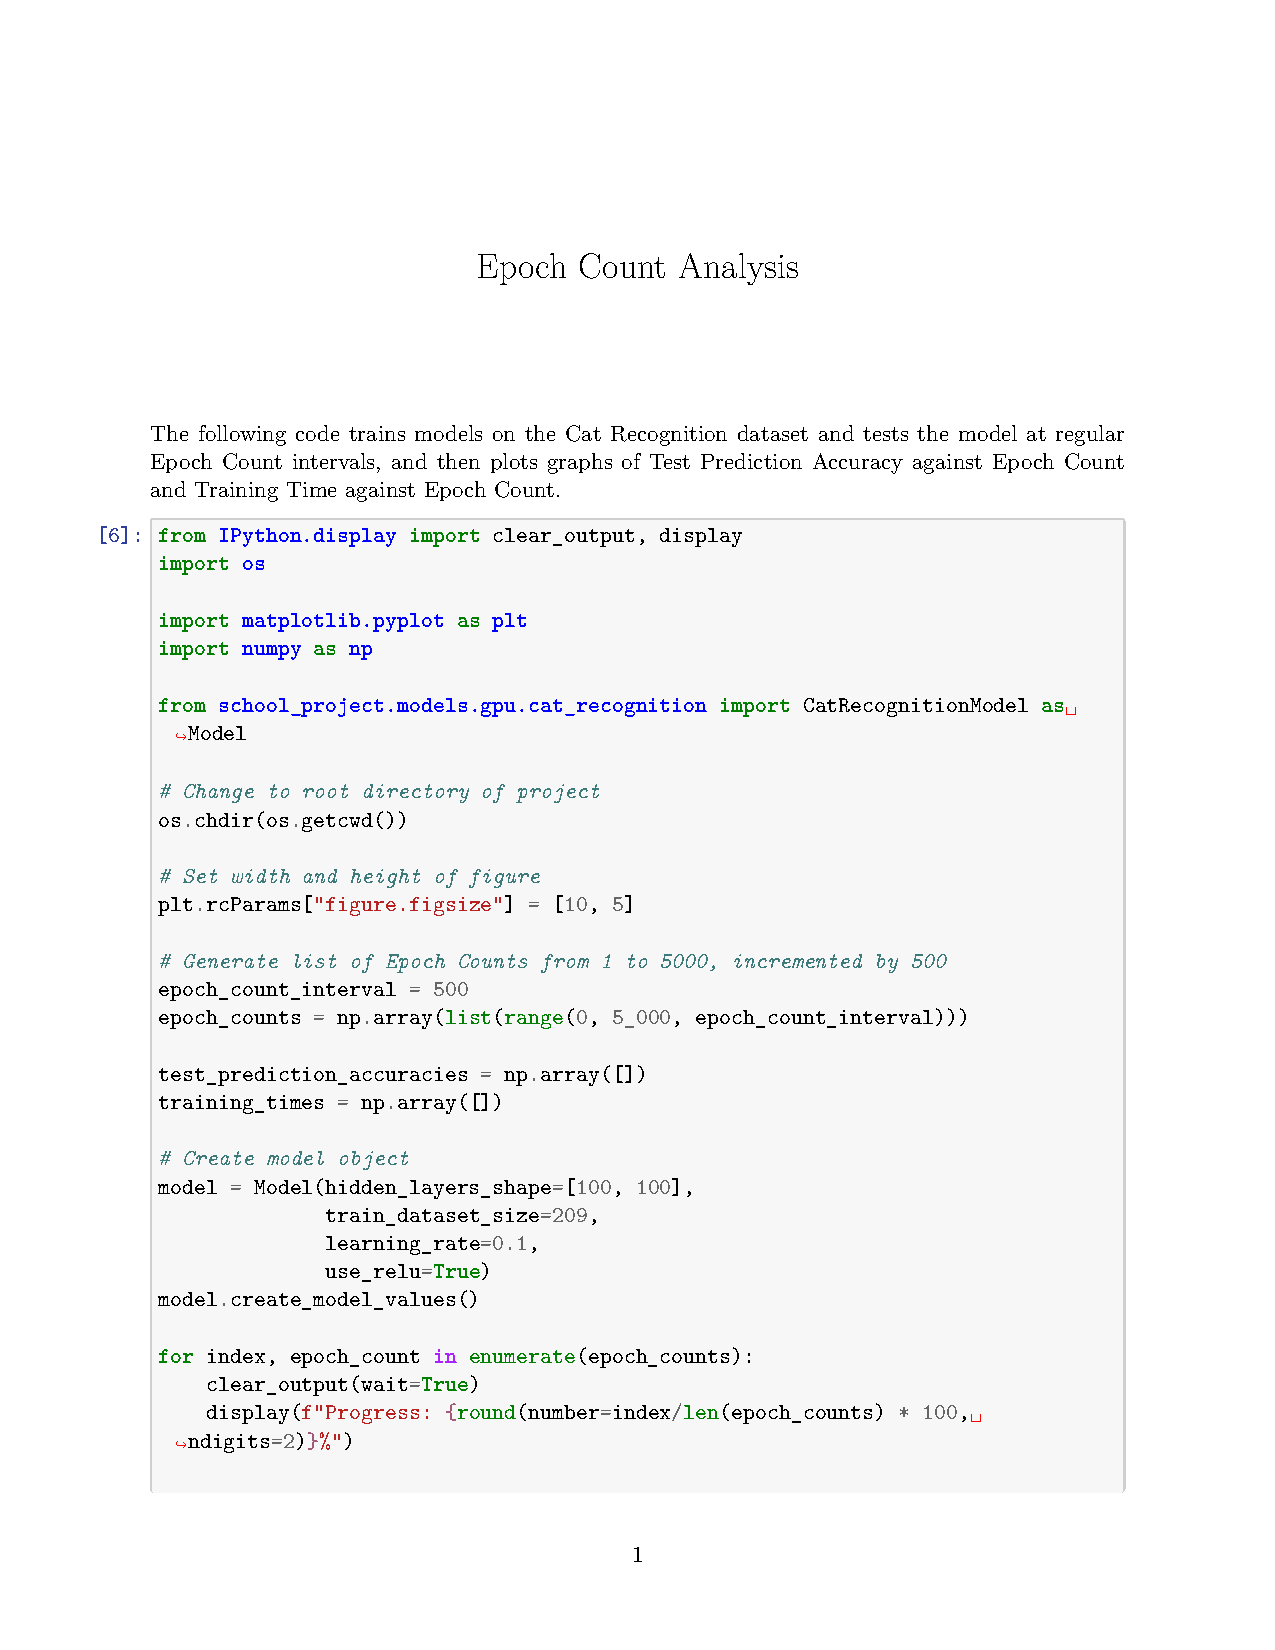
\includepdf[pages=-, pagecommand={\thispagestyle{plain}}, scale=0.9]{./project-report/src/pdfs/epoch-count-analysis.pdf}

\label{sec:train-dataset-size-analysis}

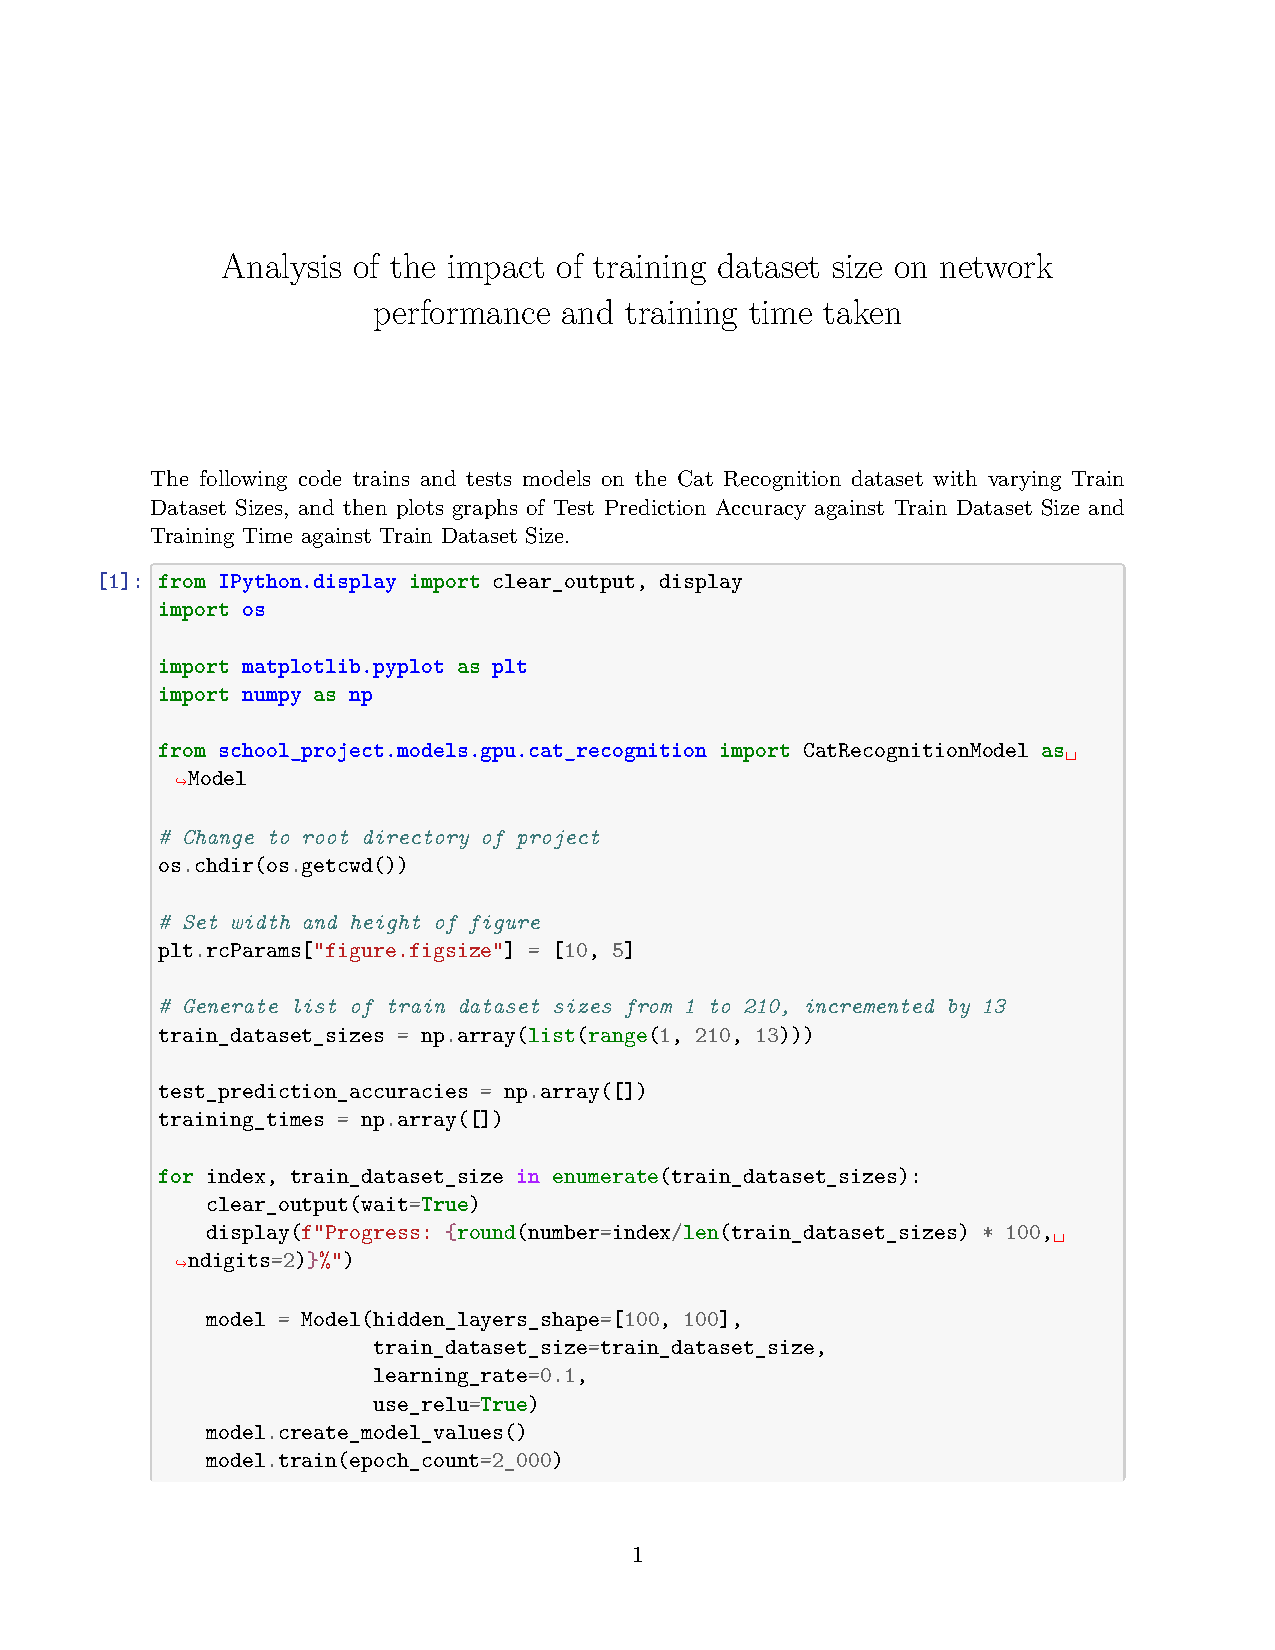
\includepdf[pages=-, pagecommand={\thispagestyle{plain}}, scale=0.9]{./project-report/src/pdfs/train-dataset-size-analysis.pdf}

\label{sec:layer-count-analysis}

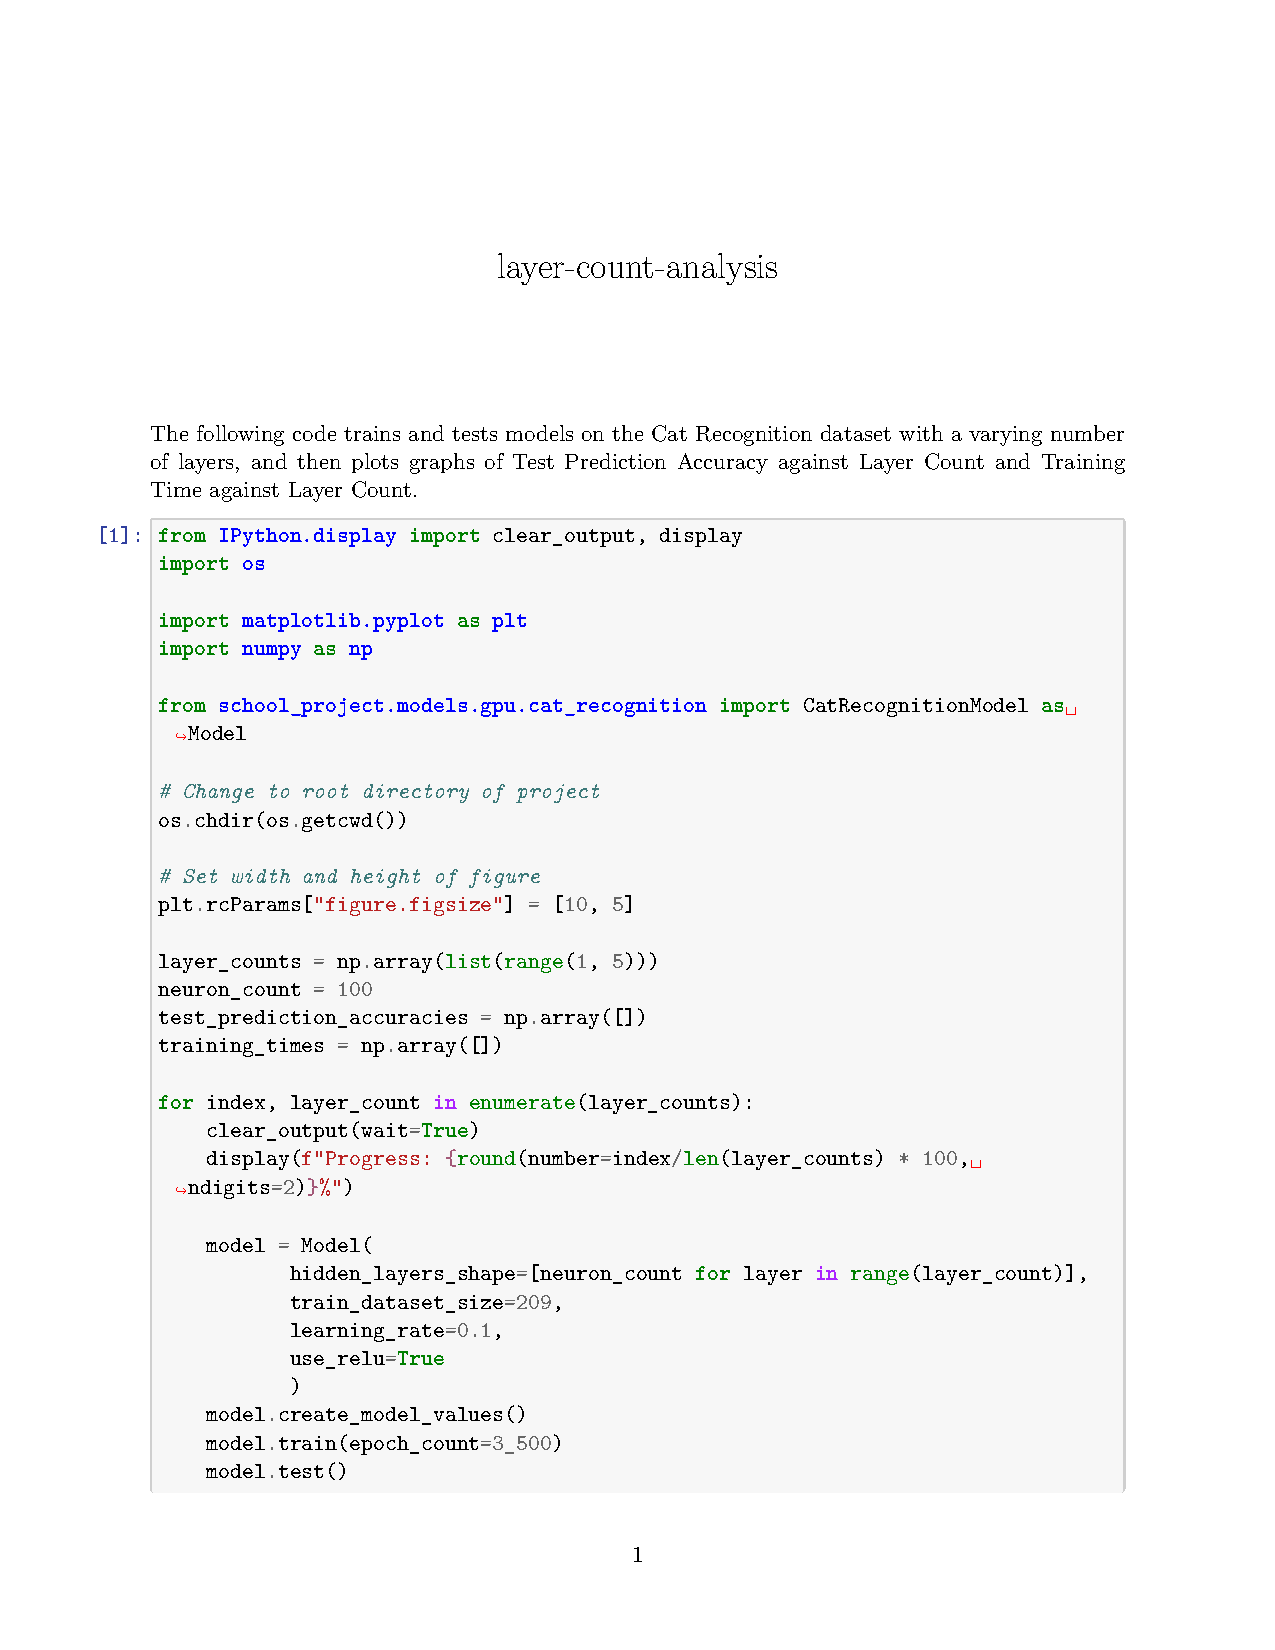
\includepdf[pages=-, pagecommand={\thispagestyle{plain}}, scale=0.9]{./project-report/src/pdfs/layer-count-analysis.pdf}

\label{sec:neuron-count-analysis}

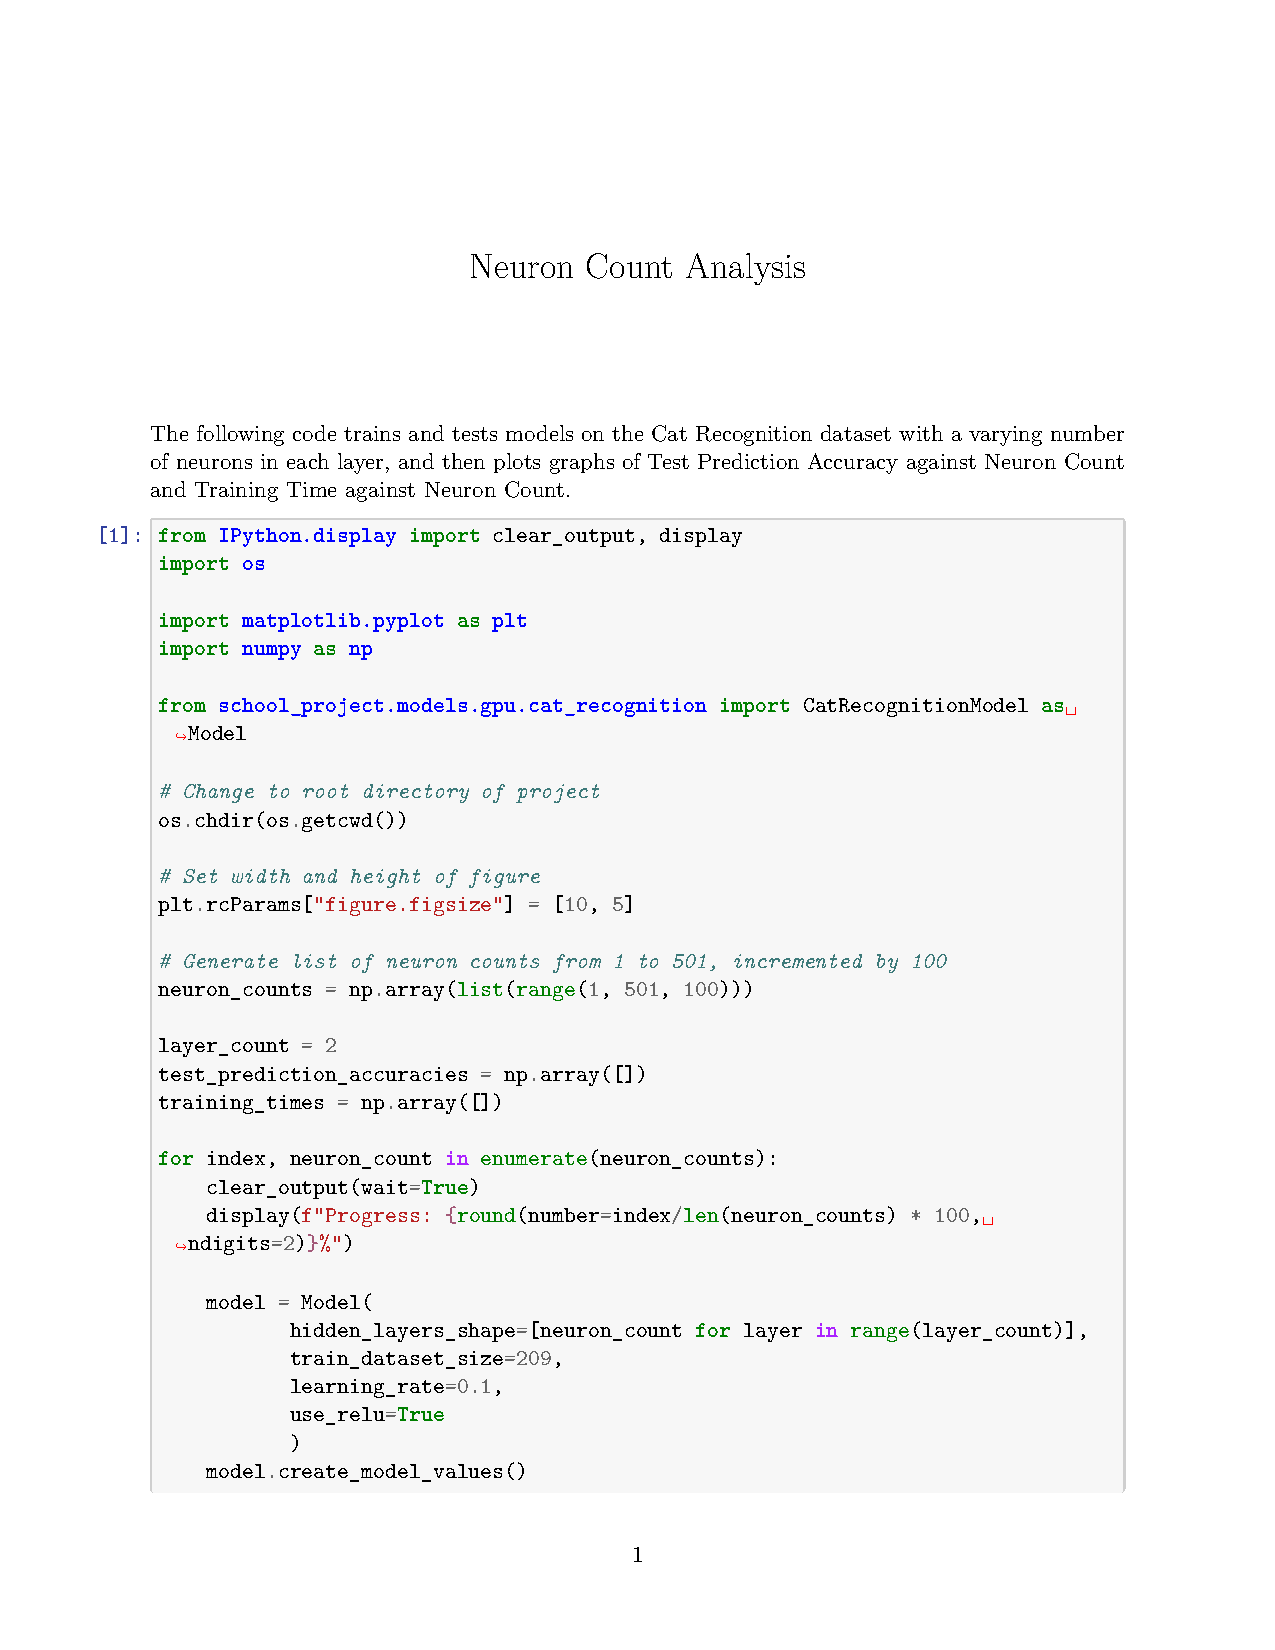
\includepdf[pages=-, pagecommand={\thispagestyle{plain}}, scale=0.9]{./project-report/src/pdfs/neuron-count-analysis.pdf}

\label{sec:relu-analysis}

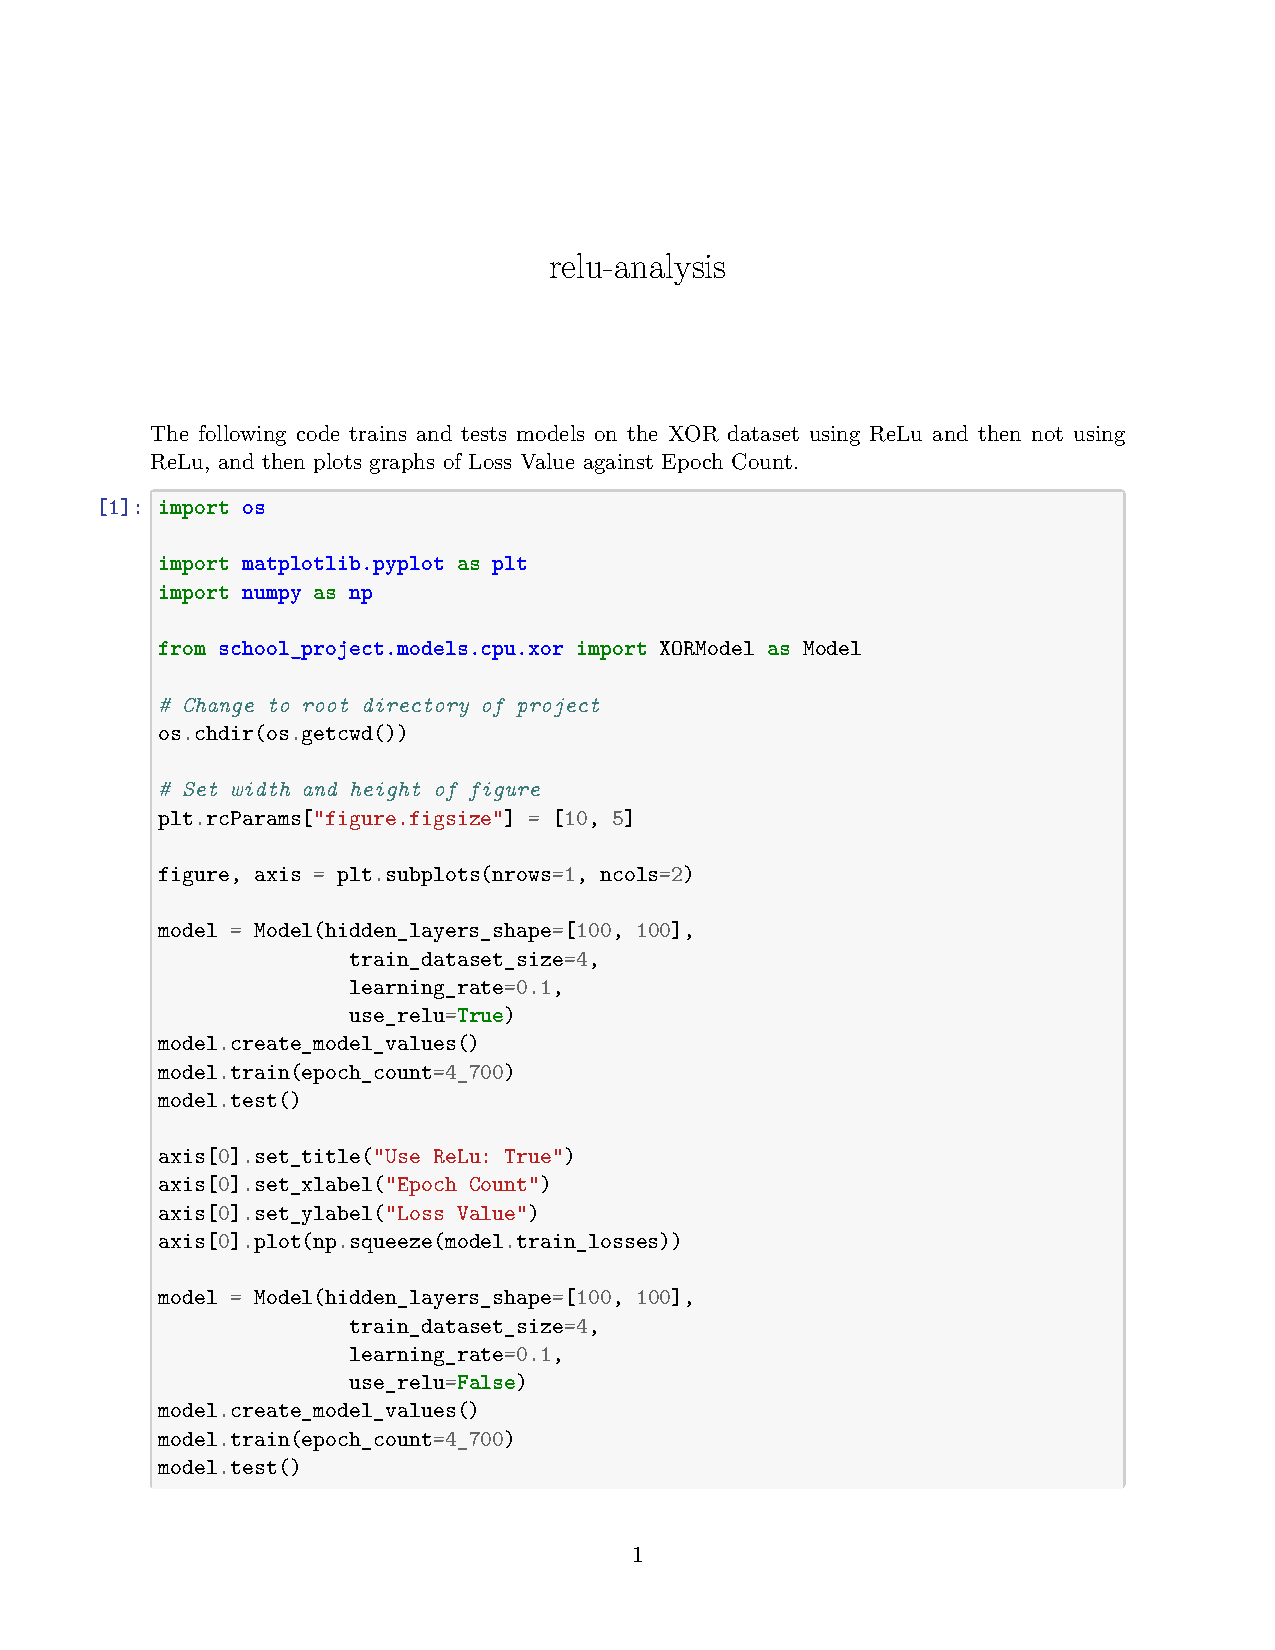
\includepdf[pages=-, pagecommand={\thispagestyle{plain}}, scale=0.9]{./project-report/src/pdfs/relu-analysis.pdf}

\label{sec:cpu-vs-gpu-analysis}

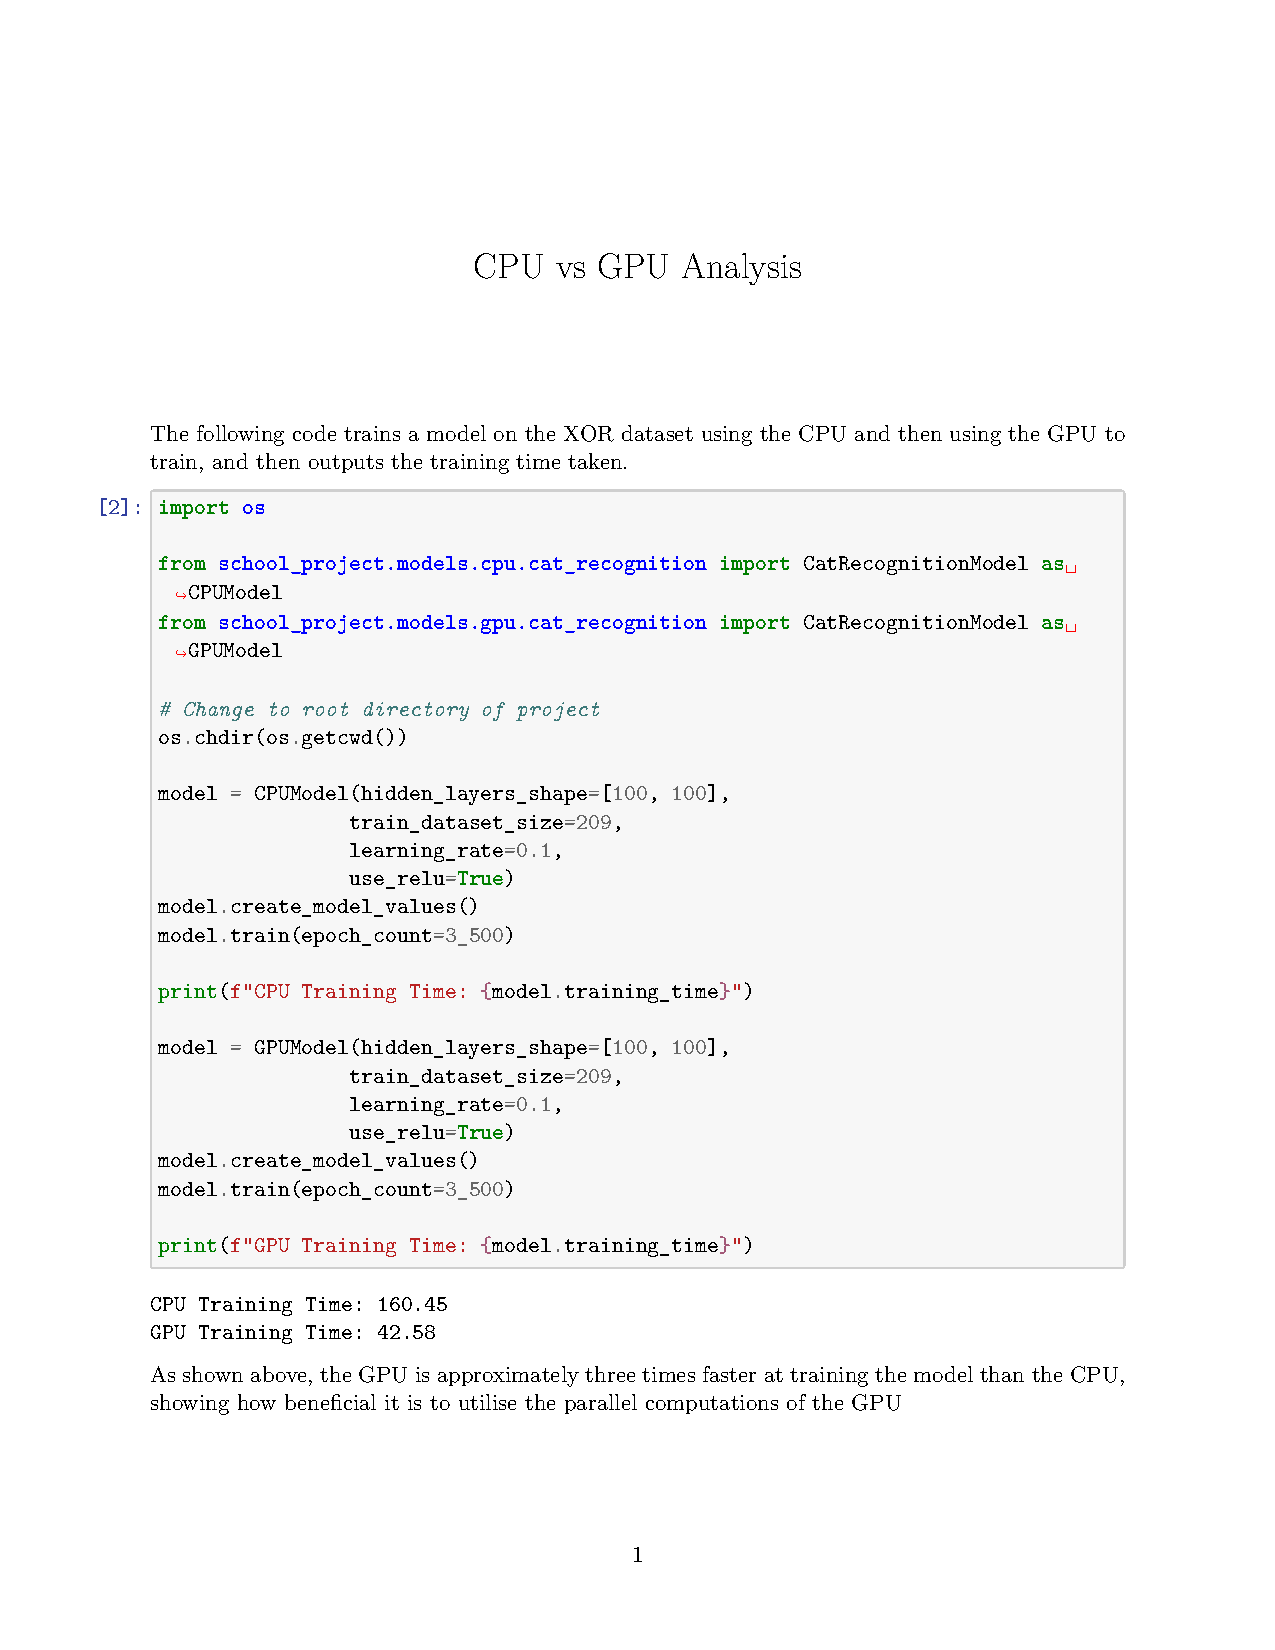
\includepdf[pages=-, pagecommand={\thispagestyle{plain}}, scale=0.9]{./project-report/src/pdfs/cpu-vs-gpu-analysis.pdf}

\subsubsection{Conclusions}

The principle conclusion from this analysis is that both the shape of the network and selection of other hyper-parameters is critical to develop an optimum Artificial Neural 
Network. 

Firstly, when considering the shape of the network, higher numbers of neurons per layer and higher layer counts do not necessarily equate to an increase in network 
performance. As can be seen on page \pageref{sec:neuron-count-analysis}, increasing neuron count passes through an ideal value before prediction accuracy begins to drop. In a 
similar manner, as can be seen on page \pageref{sec:layer-count-analysis}, increasing the number of layers passes through an optimum value before performance decreases. Both 
of these behaviours are likely due to overfitting of the network to the training dataset and was an outcome predicted during the interview I undertook at the beginning of the 
project. In fact, it was described to me that finding the optimum network shape is part analysis and part trial and error.

Secondly, key parameters within the forward and backward propagation methods have an impact on network performance. Most importantly, is the learning rate where selecting too 
small a value results in an increase in required epochs and training time - the model is also at risk of converging on a local minimum resulting in a suboptimal conclusion. 
Alternatively, selecting too high a learning rate can lead to an oscillation around the optimal solution. The nature of the transfer function similarly has a significant 
effect, with the ReLu transfer function reaching a lower loss value faster - it should be noted that the Sigmoid function did also converge but required more epochs.

With regard to the size of the training dataset, a larger dataset does appear to generate a better solution. I would expect the effect of this to reduce with a significant 
training dataset size but the size of the training dataset for Cat recognition did not reach this level.

Lastly the use of a GPU decreased training time by approximately a factor of 4, which is the result of the GPU architecture being optimized for matrix calculations.

\pagebreak

\end{document}
